\documentclass[12pt]{article}
\usepackage{ling}
\usepackage[hmargin=2.54cm,vmargin=2.54cm]{geometry}
\geometry{a4paper}
\usepackage{fancyhdr} % This should be set AFTER setting up the page geometry
\pagestyle{fancy} % options: empty , plain , fancy
\renewcommand{\headrulewidth}{0pt} % customise the layout...
\lhead{}\chead{}\rhead{}
\lfoot{}\cfoot{\thepage}\rfoot{}

\begin{document}
	\begin{center}
		\Large{\textbf{Using TextGrids in Praat}}
	\end{center}

\section{Overview} % (fold)
\label{sec:overview}

\subsection{What is a TextGrid?} % (fold)
\label{sub:what_is_a_TextGrid_}

A TextGrid is an \emph{object} used in Praat for labeling some kind of file (usually a spectrogram of a recording). It might be helpful to think of it as bullet points that correspond to important information about your sound file. In other words, a TextGrid is a type of labeling system used in Praat to organize your sound files. 


% subsection what_is_a_TextGrid_ (end)

\subsection{What is a TextGrid used for?} % (fold)
\label{sub:what_is_a_TextGrid_used_for_}

% subsection what_is_a_TextGrid_used_for_ (end)


TextGrids can be used for a wide range of purposes. Typically they label certain aspects of a spectrogram so that a more laborious task can be performed on it at a later point in time (i.e. automatically extract formant frequencies from the mid point of a vowel). 


\subsection{What does a TextGrid look like?} % (fold)
\label{sub:what_does_a_TextGrid_look_like_}


Below is a screenshot taken from Praat.

\begin{center}
	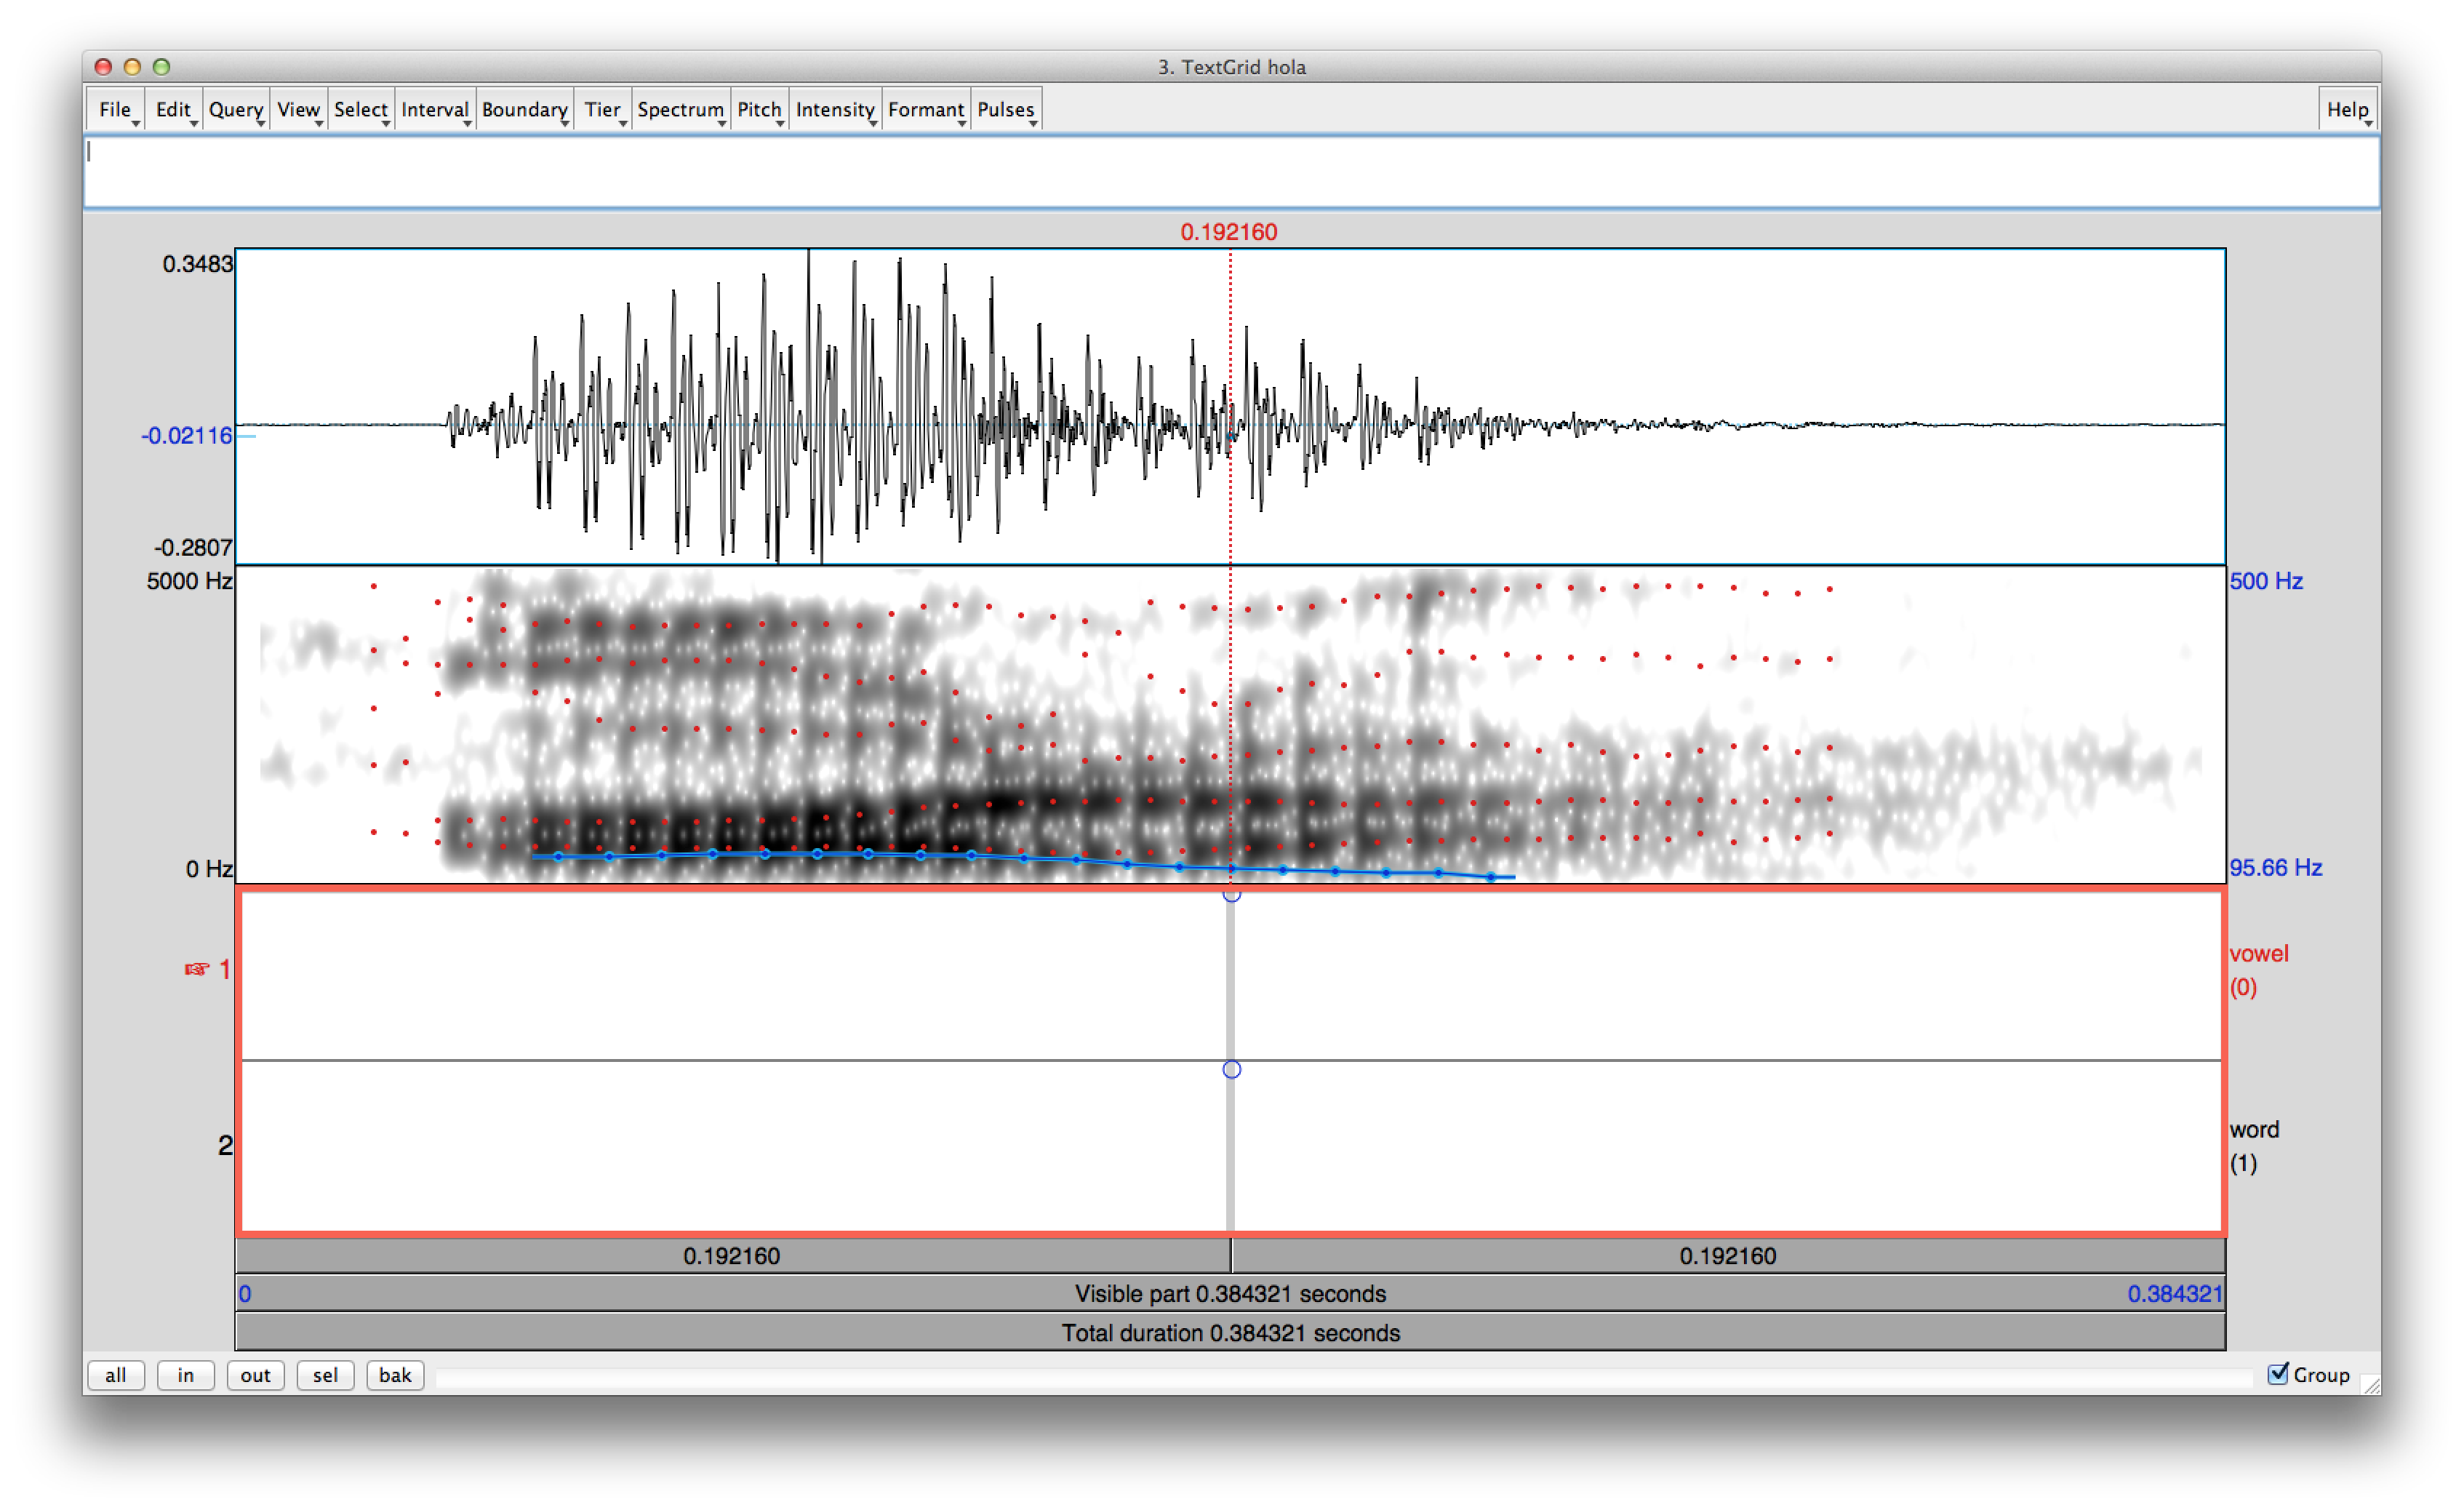
\includegraphics[scale=.12]{tg1.png}
\end{center}

Notice that in the top portion of the screenshot there is an oscillogram and a spectrogram from a recording of the word ``hola''. The TextGrid is below (outlined in red). On the left side there is finger pointing to a the number ``1'' and on the right side you can see that each \emph{tier} of the TextGrid has a corresponding name (vowel, word). You can have as many tiers as you want and can name them whatever is useful to you (avoid odd characters). Below there is an example of what a TextGrid can look like when it contains information:

\begin{center}
	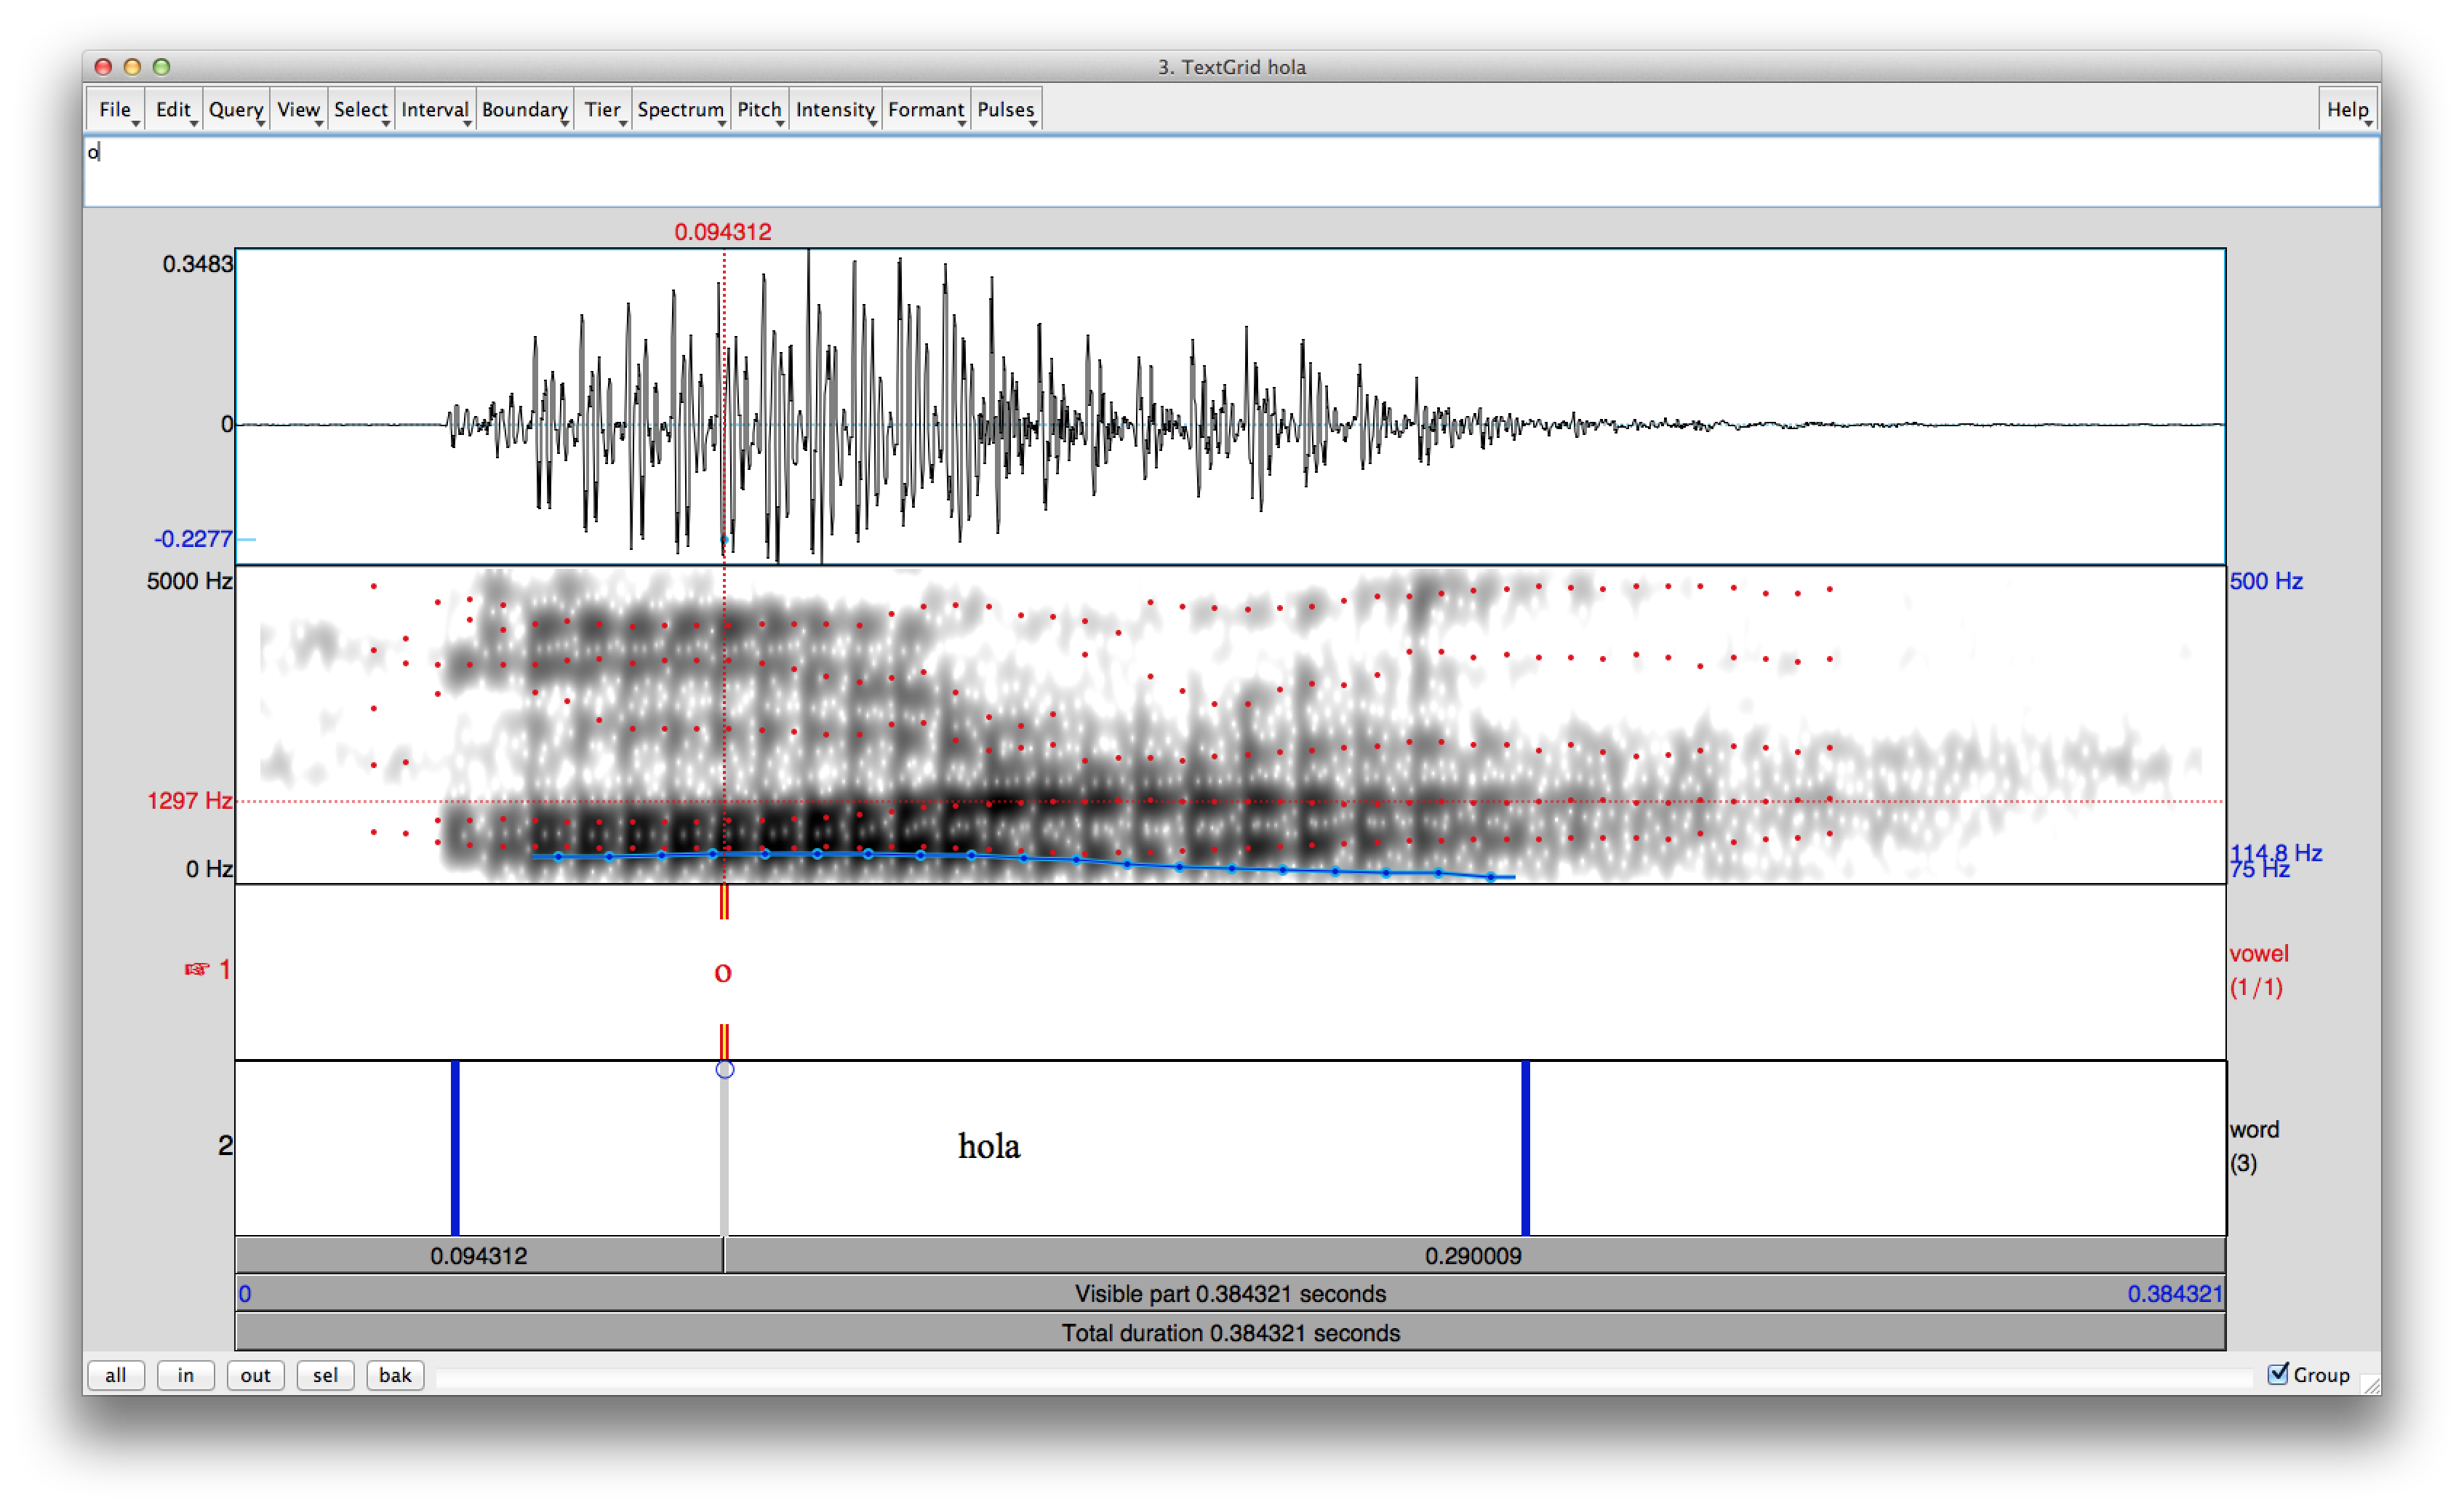
\includegraphics[scale=.12]{tg2.png}
\end{center}

Notice that the two \emph{tiers} are different. The \emph{vowel tier} has vertical broken line with the letter ``o'' in between. This could be used to label the midpoint of the vowel /o/ in the word ``hole'' (*it doesn't really correspond to the mid point but is probably close). In other words, this type of \textbf{point tier} is used to label a specific point in the spectrogram. The \emph{word tier}, on the other hand, contains two vertical, unbroken lines which mark a specific portion (or interval) of the spectrogram. This is called an \textbf{interval tier} and, in this case, is used to label the whole word ``hola''. 
% subsection what_does_a_TextGrid_look_like_ (end)
% section overview (end)

\section{Creating a TextGrid} % (fold)
\label{sec:creating_a_text_grid}

Now that you have a basic idea of what a TextGrid looks like and how it can be used, let's review how you can creat one in Praat. 

\begin{itemize}
	\item First, you need to have a ``Sound'' in the \emph{objects window}. 
	\item Next, you need to select the sound object and then click ``Annotate'' $\rightarrow$ ``To TextGrid''. 
\end{itemize}

\begin{center}
	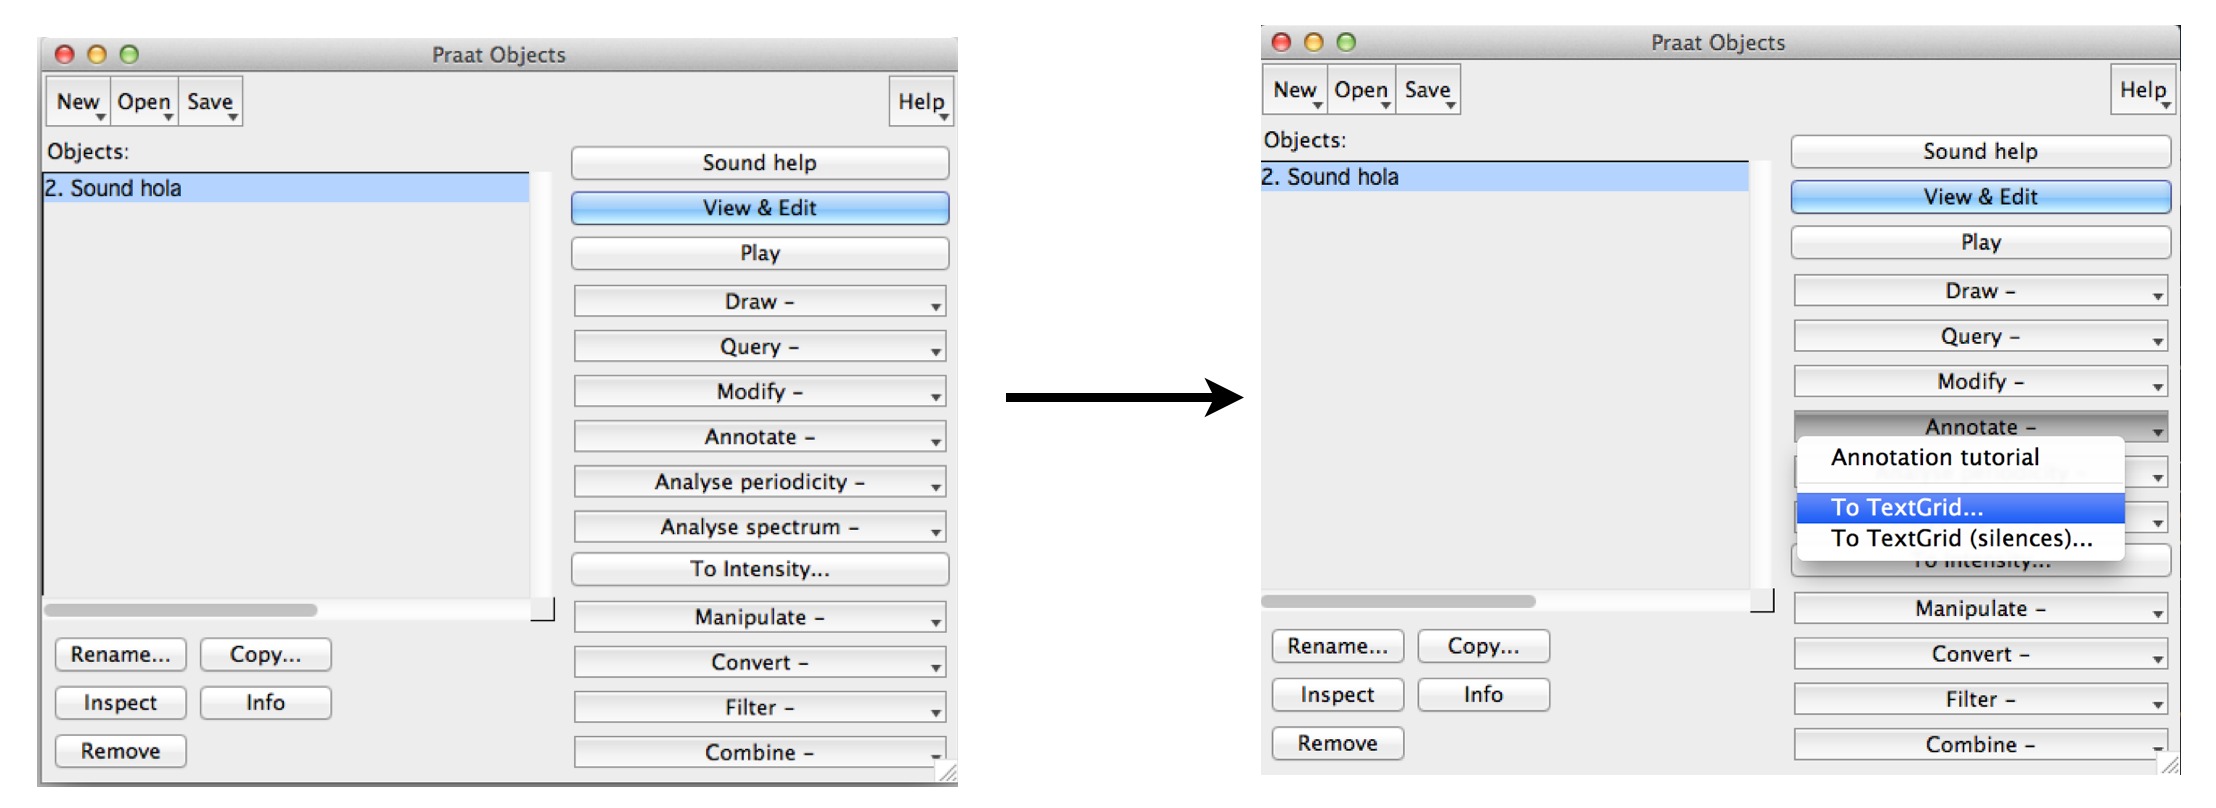
\includegraphics[scale=.4]{tg3.png}
\end{center}

\begin{itemize}
	\item This should bring up another window where you can choose the parameters of your TextGrid. 
\end{itemize}

\begin{center}
	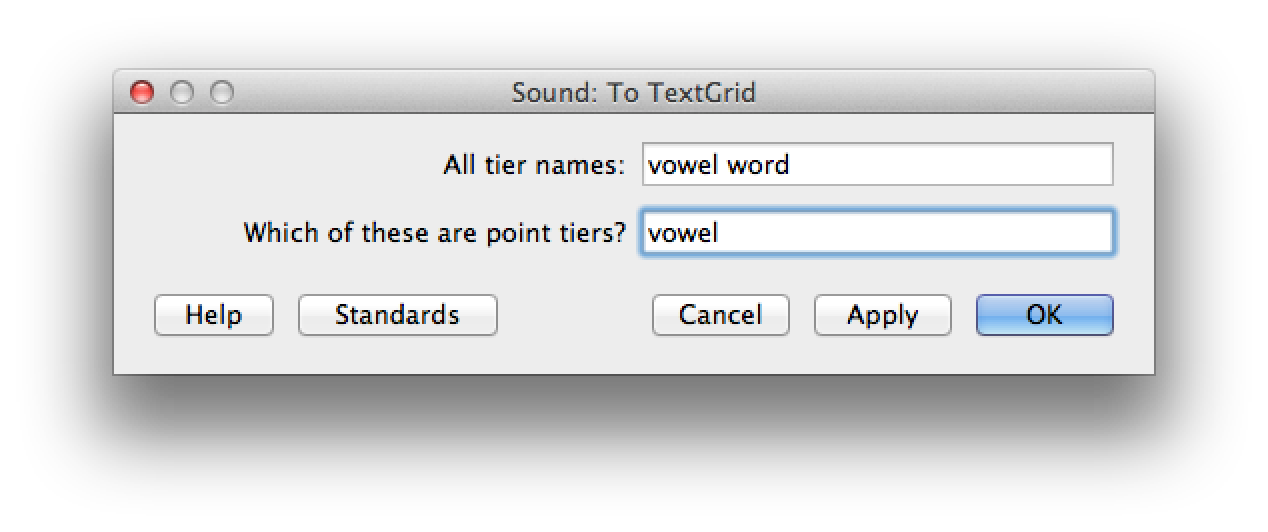
\includegraphics[scale=.25]{tg4.png}
\end{center}

\noindent The first box allows us to select the names for the tiers. Notice they are separated by a space. In this case we have a ``vowel'' tier and a ``word'' tier. The next box gives us the option to select which of the previously named tiers (vowel, word) should be point tiers. As you can see, it says ``vowel'' in this box, therefore, the vowel tier will be a point tier. The ``word'' tier will be an interval tier, which is the default if no point tier is specified. 

\begin{itemize}
	\item Finally, click ``OK'' and your TextGrid will be created and placed below the sound object in the Objects window.
\end{itemize}

\begin{center}
	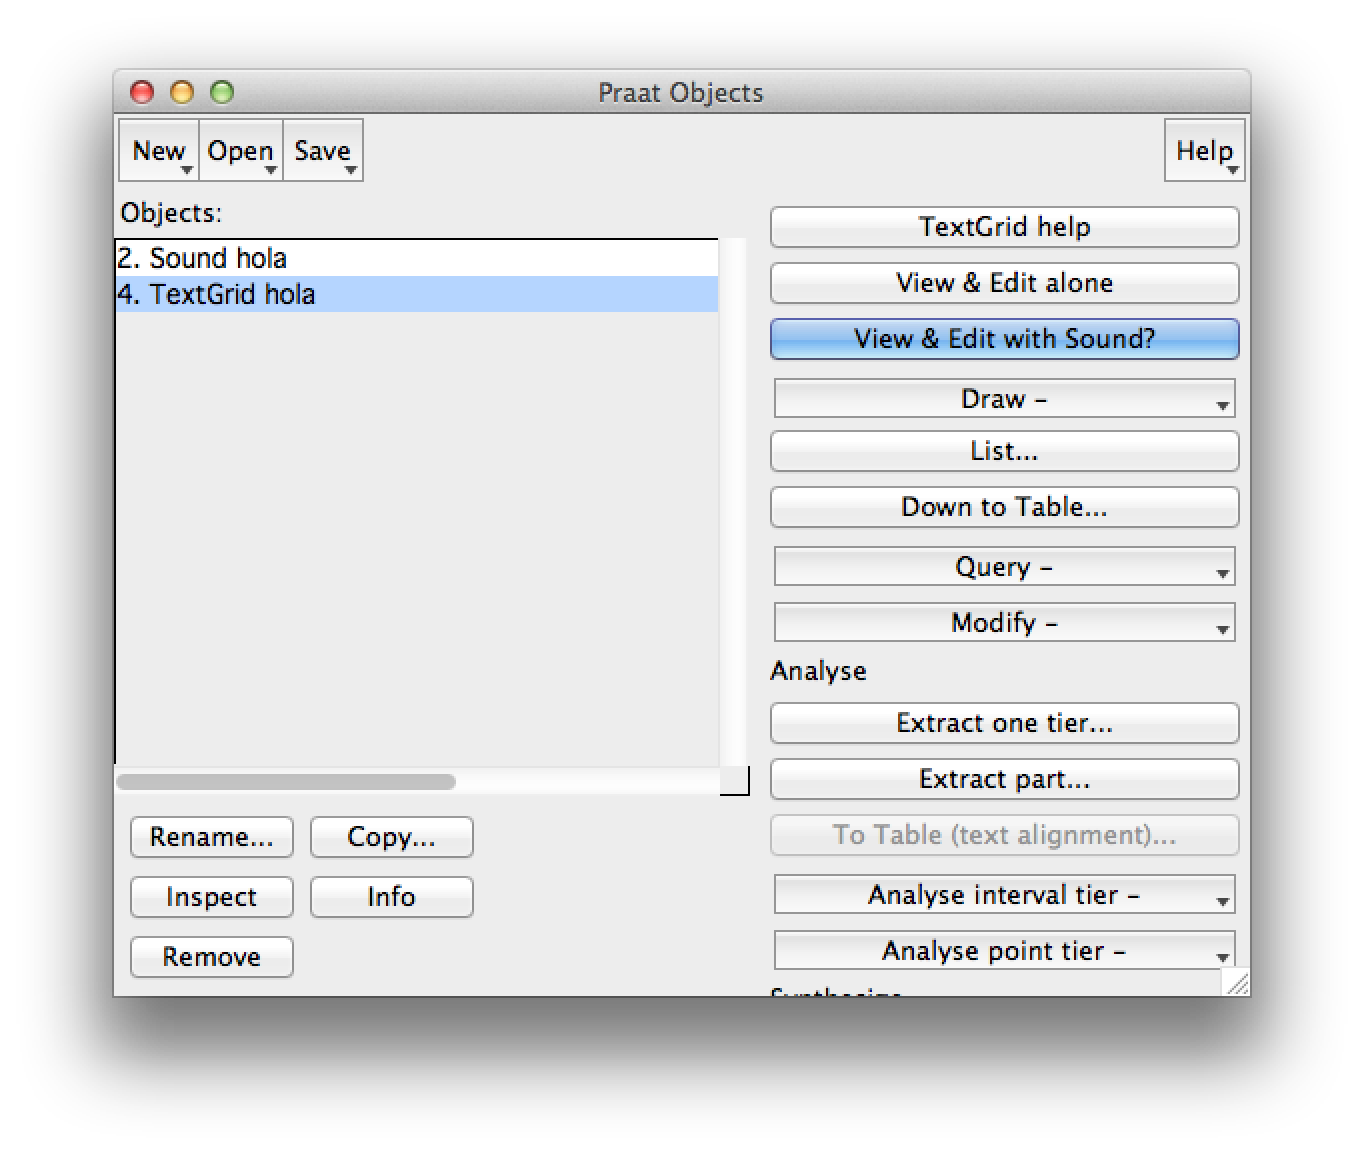
\includegraphics[scale=.28]{tg5.png}
\end{center}
% section creating_a_text_grid (end)

\section{Editing a TextGrid} % (fold)
\label{sec:editing_a_TextGrid}

In order to edit the new TextGrid \textbf{you must select both the sound object and the TextGrid} in the Object window. Doing so will change the option available in the menu on the right. Do this now. After selecting both the sound and the TextGrid, you will notice a blue button that says ``View \& Edit''. Click it to see a window similar to the first screenshot above.

Now you are ready to edit the TextGrid.  

% section editing_a_TextGrid (end)

\section{Saving a TextGrid} % (fold)
\label{sec:saving_a_TextGrid}

% section saving_a_TextGrid (end)


\section{I'm finished. Now what?} % (fold)
\label{sec:i_m_finished_now_what_}

% section i_m_finished_now_what_ (end)

\end{document}